\documentclass[lettersize,journal]{IEEEtran}
\usepackage{amsmath,amsfonts}
\usepackage{algorithmic}
\usepackage{algorithm}
\usepackage{array}
\usepackage[caption=false,font=normalsize,labelfont=sf,textfont=sf]{subfig}
\usepackage{textcomp}
\usepackage{stfloats}
\usepackage{url}
\usepackage{verbatim}
\usepackage{graphicx}
\usepackage{cite}
\hyphenation{op-tical net-works semi-conduc-tor IEEE-Xplore}
% updated with editorial comments 8/9/2021

\usepackage{booktabs} 
\usepackage{worldflags}
\flagsdefault[width=6pt, length=9pt, framewidth=0.1mm]

\begin{document}
\title{Analyzing social networks in the European Parliament, and changes in the social network over time}

\author{{BERNÁT Ádám, MARITS Márton}
        % <-this % stops a space
%\thanks{This paper was produced by deez nuts. They are in your mom.}% <-this % stops a space
%\thanks{Manuscript received June 20, 2023; published two seconds later.}
}

% The paper headers
\markboth{Journal of BME Témalabor,~Vol.~1, No.~1, June~2023}%
{Shell \MakeLowercase{\textit{et al.}}: A Sample Article Using IEEEtran.cls for IEEE Journals}

%\IEEEpubid{0000--0000/00\$00.00~\copyright~2021 IEEE}
% Remember, if you use this you must call \IEEEpubidadjcol in the second
% column for its text to clear the IEEEpubid mark.

\maketitle

\begin{abstract}
	We analyze a dataset of amendment co-sponsorship in the European Parliament. From this dataset, we construct a graph representing the co-sponsorship social network of the European Parliament, and we analyze its changes over time. We consider the changes in two important parameters of the social network, cohesion and centrality. For cohesion, we use a very simple measure, simply finding the proportion of pais of MEPs who co-contributed to amendments in a given period. For centrality, we use three different centrality measures to measure the change in centrality of political groups in the EP.
	
	We find %TODO
\end{abstract}

\section{Introduction} \label{sec:intro}

The European Parliament (EP for short) is a legislative institution of the European Union, in which representatives from each of the 28 (27 after Brexit) member states vote on legistation concerning the European Union. The Parliament consists of \textit{Members of the European Parliament} (MEPs), each of whom have a well-defined country of origin and political party. The political parties of each MEP are specific to their country of origin, but parties holding similar views organize themselves into \textit{political groups}, which act as super-parties in the context of the European Parliament.

The major political groups in the EP are the European People's Party (EPP, centre-right), the Progressive Alliance of Socialists and Democrats (S\&D, left), Renew Europe (RE, liberal), the Greens–European Free Alliance (Greens/EFA, green), European Conservatives and Reformists (ECR, right), Identity and Democracy (ID, far-right) and The Left in the European Parliament (GUE/NGL, left). Representatives who do not belong to any of these groups are usually called Non-iscrits (French for `not registered'), often abbreviated as NI.

Our aim is to analyze the social networks of the European Parliament, especially its change over time in the period between 2019 and 2023. For this analysis, we consider two important measures of the social network: cohesion and centrality.

Cohesion is a measure of how well a social network is held together as a whole, how strongly is the graph of the social network connected. To measure this in a graph $G$, we introduce the \textit{cohesion} of $G$ as \[
	\text{cohesion}(G) = \frac{2e}{\binom{n}{2}}
\] where $e$ is the number of edges and $n$ is the number of vertices in $G$. This definition naturally generalizes to subgraphs of graphs, and we will use this extensively to study the cohesion of certain subgroups of MEPs, such as different political groups and different committees.

Centrality is a measure of how `central' a node is within a graph. Notably, it is not a measure of the entire social network, rather only of a single MEP. To generalize and extend the notion to entire social networks, we use the methods outlined in \cite{Centralities}.

Some analysis of social networks in the European Union has already been done in \cite{Baller} and \cite{Cherepnalkoski}. Work that is analogous to ours in the context of the United States Congress and Senate has also been seen before in \cite{Desmarais}, \cite{Fowler}, \cite{Porter} and \cite{Tanger}; while in \cite{Fischer}, Fischer et al. conducted an analysis of such co-sponsorship networks in the Swiss parliament.

The present paper is organized as follows. In Section \ref{sec:data}, we detail the dataset available to us, its perks limitations. In Section \ref{sec:method}, we go into more detail on the three defferent centrality measures used for the analysis of group centrality. We detail our results in \ref{sec:results_coh} and \ref{sec:results}, also including a variety of plots to visualize the results on cohesiveness and centrality respectively.

\section{Our data} \label{sec:data}

Our dataset was acquired directly from the European Parliament's website. It is organized as a \texttt{csv} file which contains entries for each proposed amendment to a law, with information about when the amendment was proposed, some details about the amendment, and more importantly, information about who proposed the amendment, what party they belong to, which EP group said party belongs to, and which country are they are representative of.

This data can therefore be viewed as a bipartite graph, in which one of the bipartitions consists of the MEPs, and the other consists of the proposed amendments. An MEP and an amendment are joined by an edge if and only if said MEP contributed to the amendment (\textit{sponsored} the amendment). Importantly, a single amendment may have multiple contributors, which allows us to analyze the social structure of the European Parliament as a whole.

In total, our dataset contains 750,578 entries, which is the total number of edges in this bipartite graph. The dataset has data on a grand total of 754 MEPs.

To analyze the social structure, we \textit{projected} this bipartite graph onto the set of MEPs. This procedure creates a new graph, wherein the nodes represent MEPs, and each edge connects two MEPs which have a contribution in common. (I.e. they \textit{co-sponsored} a bill.)

With this projection, a new, not necessarily bipartite graph was created, which represents the state of the social network of the European Parliament. Notably, the number of contributions in common are not considered. An edge between two MEPs in this graph might represent a single amendment they co-sponsored, or it might represent a long-lasting relationship of co-sponsorship. The projection unfortunately obscures the details of the strength of the co-sponsorship based connection.

To account for this, we also worked with a different type of projection, a \textit{weighted projection}. This modification of the projection algorithm serves to solve the problem outlined above. With a weighted projection, as previously, we create a new graph, whose nodes represent the MEPs, and connect to MEPs if they have co-sponsored a bill together. However, we also account for the number of co-contributions, which become the weight of each edge.

\section{Our methods} \label{sec:method}

Having gathered the aggregated data from between 2019 and 2023, we split the dataset into multiple smaller sets with respect to the date. We tried monthly division, but the most suitable intervals seemed to be the quarterly and the half-yearly ones. Each data set is projected onto the set of  MEPs, using these graphs to observe the group behaviors of different parties in the European Parliament. We calculated multiple different centrality measures for each group and plotted the change of these measures over time. The different centrality measures that we used were the following:

\begin{itemize}
\item \underline{Group Degree Centrality}: The group degree centrality of a group of MEPs (e.g: European People's Party) is the fraction of non-group members connected to group members.
\item \underline{Group Closeness Centrality}: Group closeness centrality of a group of MEPs is a measure of how close the group is to the other members in the graph.
\item \underline{Group Betweenness Centrality}: Group betweenness centrality of a group of MEPs is the sum of the fraction of all pairs' shortest paths that pass through any member of the given group.
\end{itemize}

These measures are very similar to their corresponding vertex versions. The correct definitions and methodologies of the group centrality measures are discussed in \cite{Centralities}

In some cases, we further considered the different committees within the European Union. Each committee consists of several MEPs and are specialized on issues arising from one specific area and making laws in relation to said area. For example, the ITRE committee stands for ``Committee on Industry, Research and Energy" and thus deals with issues related to industrial, research and energy policy. When we specified a committee, we selected MEPs from the given committee, and we considered the MEPs in the committee as the vertices of a graph.

Our expectations and presuppositions were the following. If an event, cause, phenomenon, problem, or conflict is occurring close (either geographically or economically) to the EU, those parties that are willing to step up and have more prominent agendas regarding the aforementioned event will most likely have higher group centrality ratios as they must interact with other parties and members of the European Parliament in order to further their agendas. More cooperation and willingness for discussion from a party will lead it towards a more ``central" position as it interacts with many MEPs from other parties. On the other hand, deep division surrounding an event and unwillingness to move from one's position will result in stagnation and declining centrality for the more isolated party.

\section{Results on cohesion} \label{sec:results_coh}

\section{Results on centrality} \label{sec:results}

%TODO

%\textbf{The committee-wise whole graph approach:} %ez nagyon nem angolos :(
\textbf{The first approach:} We have calculated and plotted the centralities of all major political party groups within the EU. Here are the quarterly results of the further partitioned data, in which we separated the MEPs into committees. See Figures \ref{EPP_ENVI_Q_closeness} \ref{S&D_ENVI_Q_closeness} \ref{EPP_ITRE_Q_closeness} and \ref{S&D_ITRE_Q_closeness}; here we used closeness centrality as our measure. 


\begin{figure}[h]
  \centering
  \begin{minipage}[b]{0.23\textwidth}
    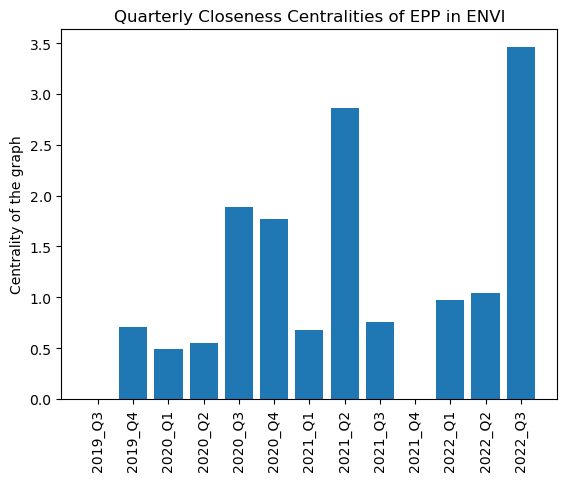
\includegraphics[width=\textwidth]{EPP_ENVI_Q_closeness.png}
    \caption{Quarterly closeness centrality of the EPP party in the ENVI committee graph}
    \label{EPP_ENVI_Q_closeness}
  \end{minipage}
  \hfill
  \begin{minipage}[b]{0.23\textwidth}
    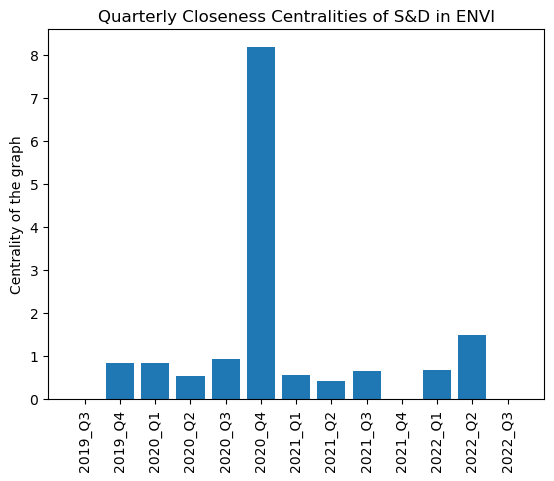
\includegraphics[width=\textwidth]{S&D_ENVI_Q_closeness.png}
    \caption{Quarterly closeness centrality of the S\&D party in the ENVI committee graph}
    \label{S&D_ENVI_Q_closeness}
  \end{minipage}
\end{figure}


\begin{figure}[h]
  \centering
  \begin{minipage}[b]{0.23\textwidth}
    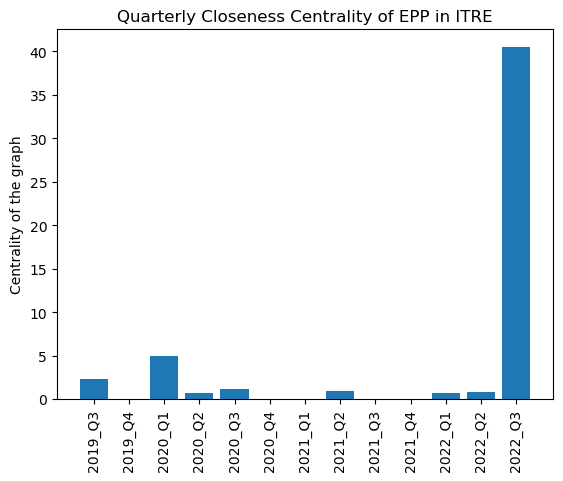
\includegraphics[width=\textwidth]{EPP_ITRE_Q_closeness.png}
    \caption{Quarterly closeness centrality of the EPP party in the ITRE committee graph}
    \label{EPP_ITRE_Q_closeness}
  \end{minipage}
  \hfill
  \begin{minipage}[b]{0.23\textwidth}
    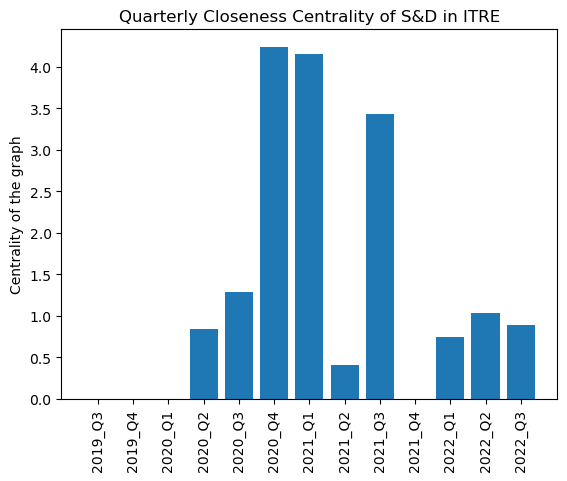
\includegraphics[width=\textwidth]{S&D_ITRE_Q_closeness.png}
    \caption{Quarterly closeness centrality of the S\&D party in the ITRE committee graph}
    \label{S&D_ITRE_Q_closeness}
  \end{minipage}
\end{figure}

The abbreviations correspond to two prominent committees:\\
ITRE: Committee on Industry, Research and Energy\\
ENVI: Committee on the Environment, Public Health and Food Safety

It is also worth noting that a centrality may be zero either because a committee did not work during a given time period or because the resulting graph is so fractured that it is not connected. %TODO

Some similar graphs are presented in Figures \ref{fig:btw_EPP} and \ref{fig:btw_S&D}; the difference is that in this case, the centrality measure is betwenness centrality.

\begin{figure}[h]
  \centering
  \begin{minipage}[b]{0.23\textwidth}
    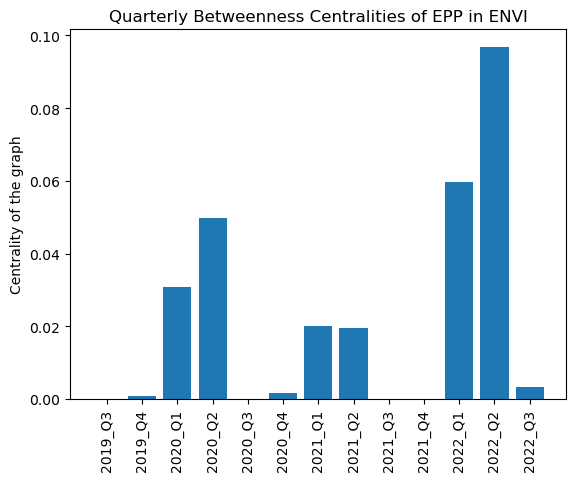
\includegraphics[width=\textwidth]{EPP_ENVI_Q_betweenness.png}
    \caption{Quarterly betweenness centrality of the EPP party in the ENVI committee graph}
    \label{fig:btw_EPP}
  \end{minipage}
  \hfill
  \begin{minipage}[b]{0.23\textwidth}
    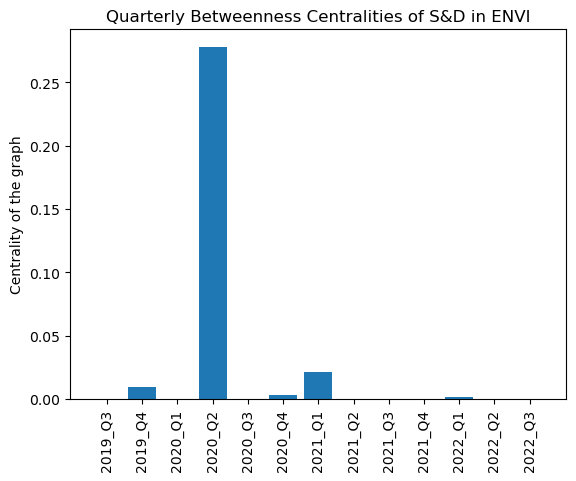
\includegraphics[width=\textwidth]{S&D_ENVI_Q_betweenness.png}
    \caption{Quarterly betweenness centrality of the S\&D party in the ENVI committee graph}
    \label{fig:btw_S&D}
  \end{minipage}

\end{figure}

The results are hardly decipherable, which we believe can be attributed to two major factors: 
\begin{itemize}
\item First, the data is too far stretched, creating uneven graphs with many components, and in a graph with many components, centralities are relatively meaningless when compared to centralities in a much larger graph.
\item Second, the individual committees often focus on their respective areas, so big spikes most likely indicate that an important agenda is on the table; while a lack of agendas will result in a lower centrality value.
\end{itemize}

%\textbf{The committee-wise greatest component approach:}
\textbf{The second approach}: Again, we restricted ourselves to one committee at a time and considered the greatest component of the connectivity graph of the MEPs. The centrality measurements were made on this giant component; in Figures \ref{EPP_ENVI_Q_closeness_BIG} \ref{S&D_ENVI_Q_closeness_BIG} \ref{EPP_ITRE_Q_closeness_BIG} and \ref{S&D_ITRE_Q_closeness_BIG}. We used group closeness centrality as the measure of centrality in this case.

\begin{figure}[h]
  \centering
  \begin{minipage}[b]{0.23\textwidth}
    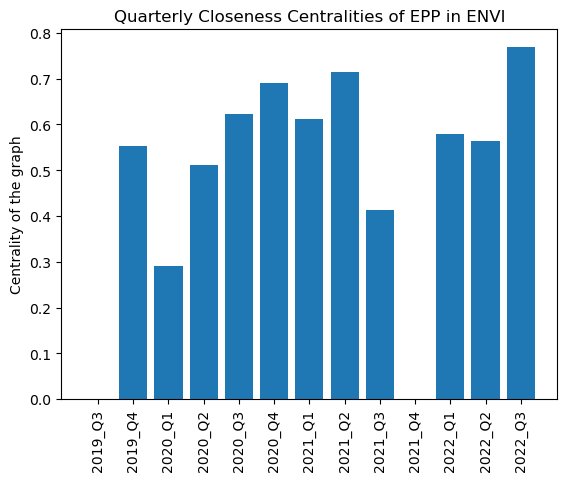
\includegraphics[width=\textwidth]{EPP_ENVI_Q_closeness_BIG.png}
    \caption{Quarterly closeness centrality of the EPP party in the  biggest component of the ENVI committee graph}
    \label{EPP_ENVI_Q_closeness_BIG}
  \end{minipage}
  \hfill
  \begin{minipage}[b]{0.23\textwidth}
    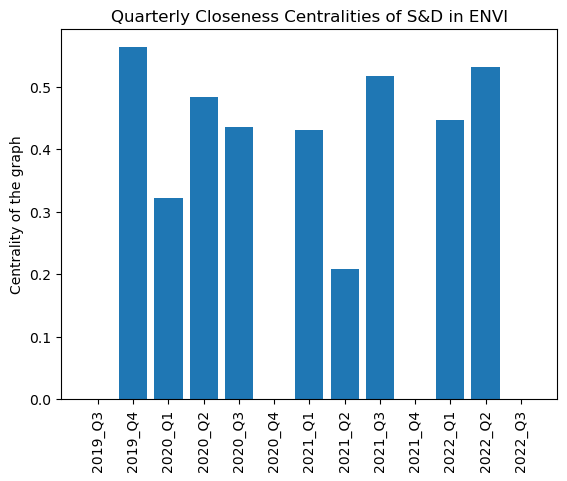
\includegraphics[width=\textwidth]{S&D_ENVI_Q_closeness_BIG.png}
    \caption{Quarterly closeness centrality of the S\&D party in the biggest component of the ENVI committee graph}
    \label{S&D_ENVI_Q_closeness_BIG}
  \end{minipage}
\end{figure}


\begin{figure}[h]
  \centering
  \begin{minipage}[b]{0.23\textwidth}
    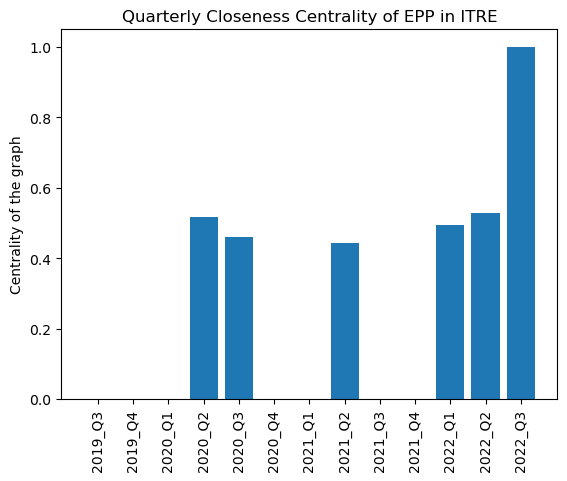
\includegraphics[width=\textwidth]{EPP_ITRE_Q_closeness_BIG.png}
    \caption{Quarterly closeness centrality of the EPP party in the biggest component of the ITRE committee graph}
    \label{EPP_ITRE_Q_closeness_BIG}
  \end{minipage}
  \hfill
  \begin{minipage}[b]{0.23\textwidth}
    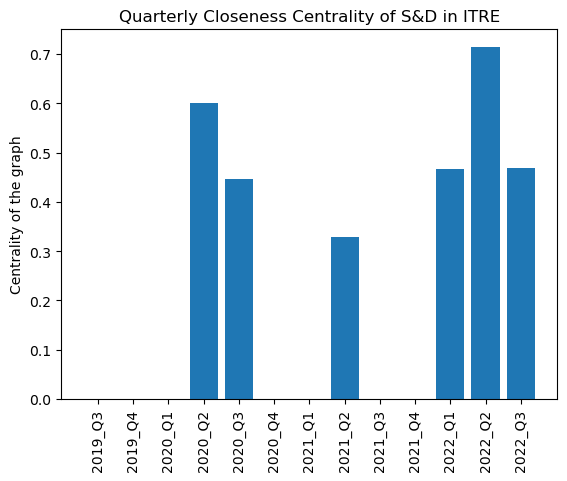
\includegraphics[width=\textwidth]{S&D_ITRE_Q_closeness_BIG.png}
    \caption{Quarterly closeness centrality of the S\&D party in the  biggest component of the ITRE committee graph}
    \label{S&D_ITRE_Q_closeness_BIG}
  \end{minipage}
\end{figure}

Observing the graphs, there seems to be an increase in activity of the ITRE committee in the second and third quarters of 2022; the group centralities are higher than before. We believe that this increase is caused by the planning of sanctions on Russia due to the Russo-Ukrainian war, and discussion related to the energy crisis that arose due to the conflict.
%This might be an indicator of the sanction planning for and the energy price consequences of the Russian-Ukranian conflict.

These graphs show more clear trends, but there are still many data points with zero centrality, which we attribute to the sparseness of edges between MEPs, which is caused by filtering the data points to the specific group of MEPs that we are investigating. 

%\textbf{The greatest component approach for the half-yearly MEP graphs:}
%TODO
\textbf{The third approach}: A different approach would be of use even more robust time periods, and no committee filter should be placed on the members. Thus, a more telling tale emerged when observing the half-yearly samples of the complete MEP structure. Similarly to the previous approach, here we also only considered the biggest components of the MEP graphs. 

On Figures \ref{EPP_HY_deg} and \ref{EPP_HY_cls}, we have plotted the degree and closeness centralities of the EPP group, respectively.

\begin{figure}[h]
  \centering
  \begin{minipage}[b]{0.23\textwidth}
    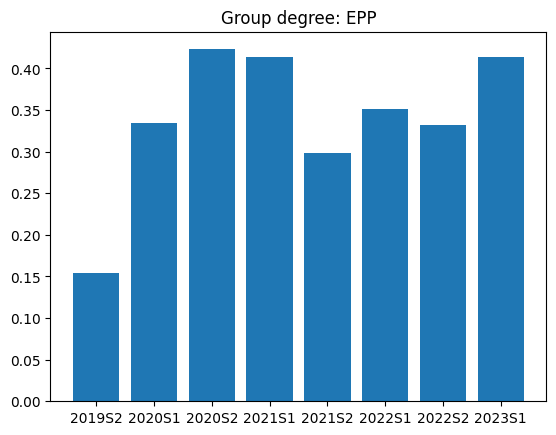
\includegraphics[width=\textwidth]{EPP_HY_deg.png}
    \caption{Half-yearly degree centrality of the EPP party in the biggest component of the MEP graph}
    \label{EPP_HY_deg}
  \end{minipage}
  \hfill
  \begin{minipage}[b]{0.23\textwidth}
    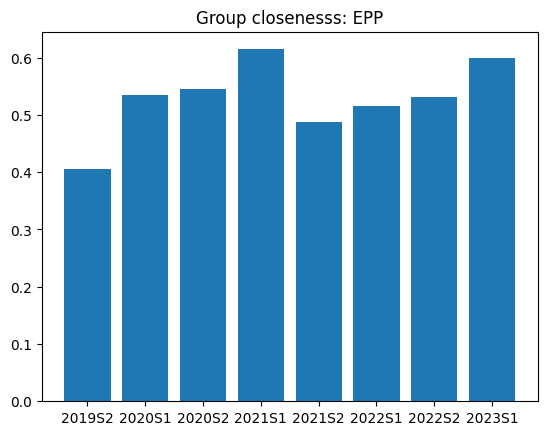
\includegraphics[width=\textwidth]{EPP_HY_cls.png}
    \caption{Half-yearly closeness centrality of the EPP party in the  biggest component of the MEP graph}
    \label{EPP_HY_cls}
  \end{minipage}
\end{figure}

Similarly, Figures \ref{S&D_HY_deg} and \ref{S&D_HY_cls} show the degree and closeness centralities of the S\&D group.

\begin{figure}[h]
  \centering
  \begin{minipage}[b]{0.23\textwidth}
    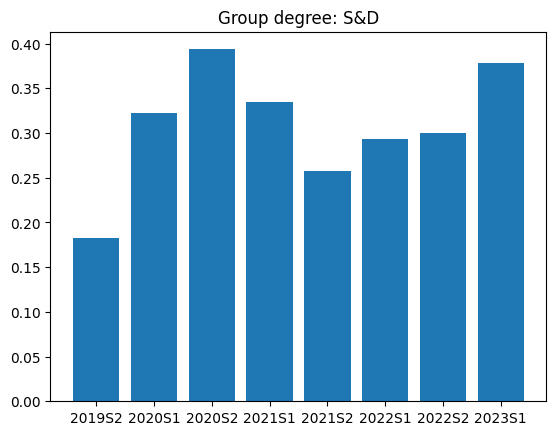
\includegraphics[width=\textwidth]{S&D_HY_deg.png}
    \caption{Half-yearly degree centrality of the S\&D party in the biggest component of the MEP graph}
    \label{S&D_HY_deg}
  \end{minipage}
  \hfill
  \begin{minipage}[b]{0.23\textwidth}
    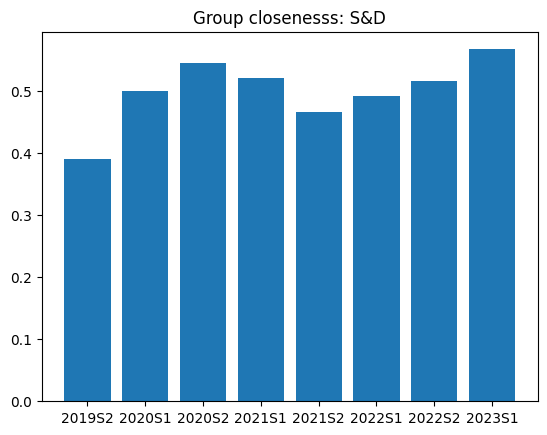
\includegraphics[width=\textwidth]{S&D_HY_cls.png}
    \caption{Half-yearly closeness centrality of the S\&D party in the  biggest component of the MEP graph}
    \label{S&D_HY_cls}
  \end{minipage}
\end{figure}

Lastly, Figures \ref{ID_HY_deg} and \ref{ID_HY_cls} show the degree and closeness centralities of the ID group in the graphs. The ID is considered a far-right or heavily right-leaning party within the European Parliament.

\begin{figure}[h]
  \centering
  \begin{minipage}[b]{0.23\textwidth}
    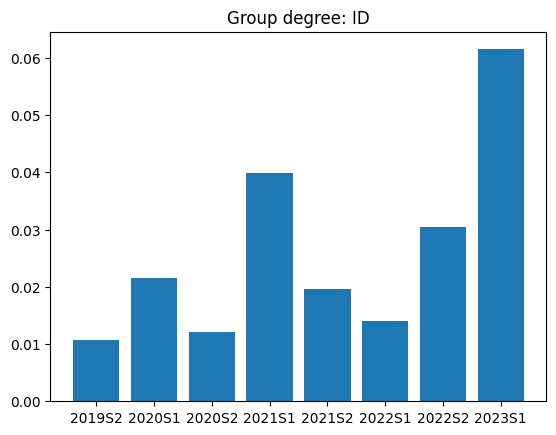
\includegraphics[width=\textwidth]{ID_HY_deg.png}
    \caption{Half-yearly degree centrality of the ID party in the biggest component of the MEP graph}
    \label{ID_HY_deg}
  \end{minipage}
  \hfill
  \begin{minipage}[b]{0.23\textwidth}
    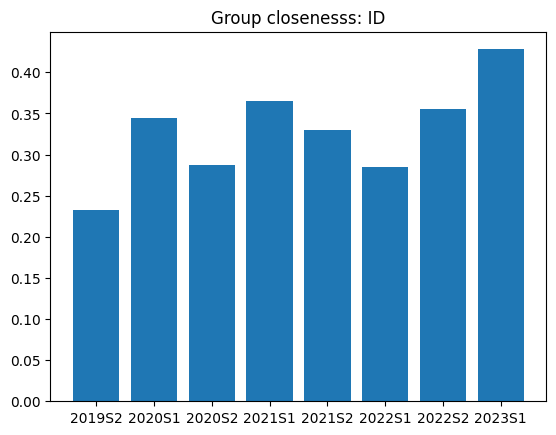
\includegraphics[width=\textwidth]{ID_HY_cls.png}
    \caption{Half-yearly closeness centrality of the ID party in the  biggest component of the MEP graph}
    \label{ID_HY_cls}
  \end{minipage}
\end{figure}

\section{Conclusions} \label{sec:conclusions}

The committee-wise analysis seems to have broken up the graph into too many pieces, thus many non-perfect results were calculated. Still, a noticeable trend is in the activity of the ITRE committee that we have touched on in the previous section. This might be an indicator of the lawmaking process and response to the effects of the Russian-Ukraine war and the consequent energy crisis. 

While the different centrality measures were not always able to produce a meaningful number, the more robust approach in the latter part ensured that the centrality measures were always positive, and there were no data points missing due to insufficient amounts of data. %no 0 measure was given to these parties. 

While S\&D is generally considered left-leaning and the EPP is right-leaning, still, they are the moderate parties and the most populous ones. Mostly stagnation can be observed; a slight increase in centralities in recent years is also noticeable. Whereas, the ID is considered a far-right party, and its centralities seem to have increased more dramatically. While this is no strong evidence, a certain affinity to increase the centralities has recently emerged in the cases of the far-right and far-left-leaning parties. These parties are still far from being very influential and really central, however, they are no longer as isolated within the parliament as they once were.

\begin{thebibliography}{1}
\bibliographystyle{IEEEtran}

\bibitem{Baller}
Baller, Inger. "Specialists, party members, or national representatives: Patterns in co-sponsorship of amendments in the European Parliament." European Union Politics 18.3 (2017): 469-490.

\bibitem{Cherepnalkoski}
Cherepnalkoski, Darko \& Mozetič, Igor. "Retweet networks of the European Parliament: Evaluation of the community structure." Applied network science 1 (2016): 1-20.

\bibitem{Desmarais}
Desmarais, Bruce A., et al. "Measuring legislative collaboration: The Senate press events network." Social Networks 40 (2015): 43-54.

\bibitem{Centralities}
Everett, Martin \& Borgatti, Stephen. (1999). The Centrality of Groups and Classes. Journal of Mathematical Sociology. 23. 181-201. 10.1080/0022250X.1999.9990219.

\bibitem{Fischer}
Fischer, Manuel, et al. "How MPs ties to interest groups matter for legislative co-sponsorship." Social networks 57 (2019): 34-42.

\bibitem{Fowler}
Fowler, James H. "Connecting the Congress: A study of cosponsorship networks." Political analysis 14.4 (2006): 456-487.

\bibitem{McPherson}
McPherson, Miller \& Smith-Lovin, Lynn \& Cook, James M. "Birds of a feather: Homophily in social networks." Annual review of sociology 27.1 (2001): 415-444.

\bibitem{Neal}
Neal, Zachary. "The backbone of bipartite projections: Inferring relationships from co-authorship, co-sponsorship, co-attendance and other co-behaviors." Social Networks 39 (2014): 84-97.

\bibitem{Peixoto}
Peixoto, Tiago P. \& Rosvall, Martin. "Modelling sequences and temporal networks with dynamic community structures." Nature communications 8.1 (2017): 582.

\bibitem{Porter}
Porter, Mason A., et al. "A network analysis of committees in the US House of Representatives." Proceedings of the National Academy of Sciences 102.20 (2005): 7057-7062.

\bibitem{Tanger}
Tanger, Shaun M. \& Laband, David N. "An empirical analysis of bill co-sponsorship in the US Senate: The Tree Act of 2007." Forest Policy and Economics 11.4 (2009): 260-265.

\end{thebibliography}


\end{document}